% Escrito del Proyecto Terminal 1 (rehecho). Compilar con:  make escrito
% Regla (1): ninguna cifra a mano. Todos los números vienen de
% ../reports/numeros.tex (generado por scripts/make_numeros.py).
\documentclass[11pt]{article}
\usepackage[spanish,es-noshorthands]{babel}
\usepackage[utf8]{inputenc}
\usepackage{amsmath,amssymb,graphicx,booktabs,hyperref}
\graphicspath{{../reports/figuras/}}

% ARCHIVO GENERADO por scripts/make_numeros.py. NO EDITAR A MANO.
% Fuente: reports/resultados/sintetico_h1.json
\newcommand{\SintB}{200}
\newcommand{\SintCasosBootRceroInf}{1.77}
\newcommand{\SintCasosBootRceroSup}{1.8}
\newcommand{\SintCasosBootReffInf}{1.48}
\newcommand{\SintCasosBootReffSup}{1.52}
\newcommand{\SintCasosMLERcero}{1.79}
\newcommand{\SintCasosMLEReff}{1.5}
\newcommand{\SintCasosMLEicero}{\ensuremath{1.36\times 10^{-5}}}
\newcommand{\SintCasosMLEk}{20.7}
\newcommand{\SintCasosMLErho}{0.0669}
\newcommand{\SintCasosMLEscero}{0.841}
\newcommand{\SintCasosPerfilRceroInf}{1.56}
\newcommand{\SintCasosPerfilRceroSup}{29.1}
\newcommand{\SintGammaInv}{7}
\newcommand{\SintMallaRceroInf}{1.1}
\newcommand{\SintMallaRceroSup}{40}
\newcommand{\SintN}{1e+07}
\newcommand{\SintRangoRceroInf}{1.5}
\newcommand{\SintRangoRceroSup}{25}
\newcommand{\SintSeroBootRceroInf}{2.46}
\newcommand{\SintSeroBootRceroSup}{2.8}
\newcommand{\SintSeroBootReffInf}{1.49}
\newcommand{\SintSeroBootReffSup}{1.52}
\newcommand{\SintSeroMLERcero}{2.6}
\newcommand{\SintSeroMLEReff}{1.5}
\newcommand{\SintSeroMLEicero}{\ensuremath{9.37\times 10^{-6}}}
\newcommand{\SintSeroMLEk}{20.7}
\newcommand{\SintSeroMLErho}{0.0973}
\newcommand{\SintSeroMLEscero}{0.578}
\newcommand{\SintSeroPerfilRceroInf}{2.45}
\newcommand{\SintSeroPerfilRceroSup}{2.74}
\newcommand{\SintVerdadRcero}{2.5}
\newcommand{\SintVerdadReff}{1.5}
\newcommand{\SintVerdadicero}{\ensuremath{1.00\times 10^{-5}}}
\newcommand{\SintVerdadk}{20}
\newcommand{\SintVerdadrho}{0.1}
\newcommand{\SintVerdadscero}{0.6}


\title{¿Qué tanto de la COVID-19 en México cabe en un SIR?\\
\large Identificabilidad, pronóstico y cambios de transmisión, 2020--2023}
\author{Ángel Omar García Hernández\\Licenciatura en Física, UAM-Iztapalapa}
\date{}

\begin{document}
\maketitle

\section{Introducción}
% PENDIENTE (F6). Pregunta, hipótesis H1--H5 y alcance: solo SIR.

\section{Modelo}
% Borrador (F2). Debe coincidir con src/sir.py y src/verosimilitud.py.
Usamos el SIR en fracciones de población,
\begin{align}
  \dot s &= -\beta s i, & \dot i &= \beta s i - \gamma i, & \beta &= R_0\gamma,
\end{align}
con $s(0)=s_0$ e $i(0)=i_0$. Los casos reportados en la semana $k$ siguen
una binomial negativa de media
\begin{equation}
  \mu_k = \rho N\,[s(t_k) - s(t_{k+1})], \qquad t_k = 7k\ \text{días},
  \label{eq:mu}
\end{equation}
y tamaño $k$, de modo que $\operatorname{Var} = \mu_k + \mu_k^2/k$.
El aumento de seroprevalencia entre los días $t_a$ y $t_b$ se modela como
$s(t_a)-s(t_b)$ con error normal de desviación igual al error estándar de
la encuesta.

\section{Identificabilidad de $R_0$ y $s_0$ (H1)}
% Borrador (F2/F4). Cifras: reports/numeros.tex. Figura: make_figuras.py.

\paragraph{Simetría de escala.}
Sea $(s,i)$ la solución con parámetros $(\beta, s_0, i_0)$ y sea $c>0$.
Las funciones $s' = s/c$, $i' = i/c$ cumplen
\begin{align*}
  \dot s' &= -\tfrac{1}{c}\beta s i = -(c\beta)\, s' i', \\
  \dot i' &= \tfrac{1}{c}(\beta s i - \gamma i) = (c\beta)\, s' i' - \gamma i',
\end{align*}
con $s'(0)=s_0/c$, $i'(0)=i_0/c$. Por unicidad, $(s',i')$ es la solución
del SIR con $(c\beta, s_0/c, i_0/c)$. Con $\rho' = c\rho$, la media
\eqref{eq:mu} no cambia:
$\rho' N [s'(t_k)-s'(t_{k+1})] = \rho N [s(t_k)-s(t_{k+1})]$.
Por lo tanto, con casos solos los parámetros
$(R_0, s_0, i_0, \rho)$ y $(cR_0, s_0/c, i_0/c, c\rho)$ son
indistinguibles para \emph{cualquier} tamaño de muestra: es una
no identificabilidad estructural. Las combinaciones invariantes son
$R_{\mathrm{eff}}(0)=R_0 s_0$, $\rho s_0$ e $i_0/s_0$. Las restricciones
$s_0\le 1$ y $\rho\le 1$ dan $s_0 \le c \le 1/\rho$, así que $R_0$ solo
queda acotado al intervalo $[R_0 s_0,\, R_0/\rho]$.

La serología rompe la simetría porque el aumento de seroprevalencia
$s(t_a)-s(t_b)$ se transforma en $[s(t_a)-s(t_b)]/c$.

\paragraph{Verificación con datos sintéticos.}
Simulamos una ola con $R_0=\SintVerdadRcero$, $s_0=\SintVerdadscero$,
$\rho=\SintVerdadrho$, $1/\gamma=\SintGammaInv$ días y
$N=\SintN$ (valores de diseño, \texttt{config/parametros.yaml}). El rango
no identificable predicho es $R_0\in[\SintRangoRceroInf,\SintRangoRceroSup]$.
Con casos solos, la MLE de $R_{\mathrm{eff}}(0)$ es $\SintCasosMLEReff$
(verdad $\SintVerdadReff$; bootstrap paramétrico con $B=\SintB$:
$[\SintCasosBootReffInf, \SintCasosBootReffSup]$). El perfil de $R_0$, en
cambio, es plano en todo el rango predicho; el intervalo de perfil
$[\SintCasosPerfilRceroInf, \SintCasosPerfilRceroSup]$ es finito, pero sus
extremos los ponen las restricciones $s_0\le1$ y $\rho\le1$, no los datos.
Por eso el criterio de no identificabilidad no puede ser ``intervalo
abierto'': hay que comparar el intervalo con el rango admisible.

Advertencia sobre el bootstrap: con casos solos, el intervalo bootstrap de
$R_0$ sale $[\SintCasosBootRceroInf, \SintCasosBootRceroSup]$, angostísimo y
sin contener la verdad. No es precisión: cada réplica se reajusta partiendo
de la MLE y el optimizador se queda donde empieza porque la verosimilitud es
plana en esa dirección. El bootstrap solo es informativo para
combinaciones identificables (como $R_{\mathrm{eff}}(0)$); por eso el
perfil va primero.

Al agregar una encuesta serológica, el intervalo de perfil de $R_0$ se
cierra en $[\SintSeroPerfilRceroInf, \SintSeroPerfilRceroSup]$ (bootstrap:
$[\SintSeroBootRceroInf, \SintSeroBootRceroSup]$), ambos conteniendo el
valor verdadero. Esto es una sola realización; la cobertura en muchas
réplicas queda para F4.

\begin{figure}[h]
  \centering
  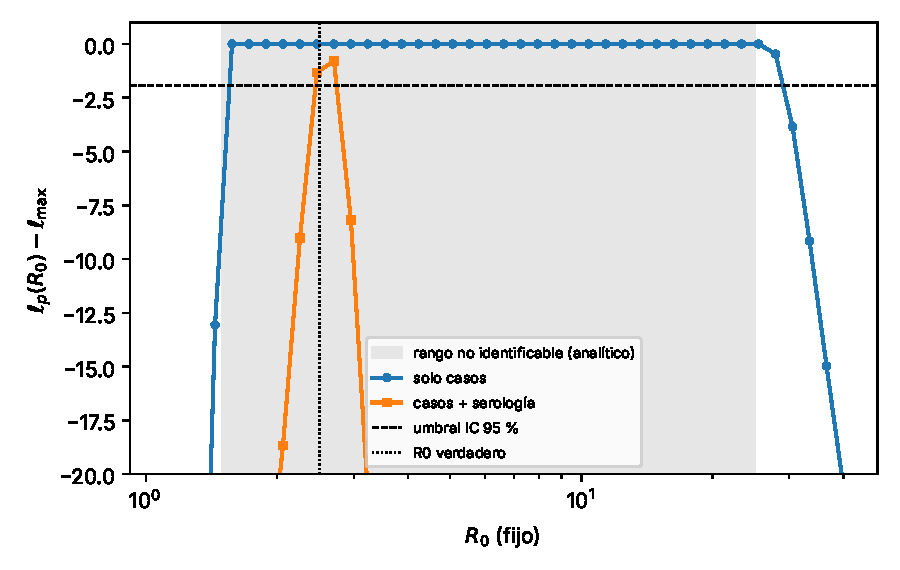
\includegraphics[width=0.8\linewidth]{perfil_R0_sintetico.pdf}
  \caption{Perfil de verosimilitud de $R_0$ en datos sintéticos. La banda
  gris es el rango no identificable predicho por la simetría de escala.
  El eje vertical se corta en $-20$; los puntos por debajo existen y están
  en \texttt{reports/resultados/sintetico\_h1.json}.}
\end{figure}

\begin{table}[h]
  \centering
  % GENERADO por scripts/make_tablas.py. NO EDITAR A MANO.
\begin{tabular}{lccc}
\hline
Parámetro & Verdad & MLE (casos) & MLE (casos + serología) \\
\hline
$R_0$ & 2.5 & 1.93 & 2.6 \\
$s_0$ & 0.6 & 0.777 & 0.578 \\
$i_0$ & \ensuremath{1.00\times 10^{-5}} & \ensuremath{1.26\times 10^{-5}} & \ensuremath{9.37\times 10^{-6}} \\
$\rho$ & 0.1 & 0.0724 & 0.0973 \\
$k$ & 20 & 20.7 & 20.7 \\
$R_{\mathrm{eff}}(0)=R_0 s_0$ & 1.5 & 1.5 & 1.5 \\
\hline
\end{tabular}

  \caption{Recuperación de parámetros en la ola sintética.}
\end{table}


\bibliographystyle{apalike}
\bibliography{../bibliografia/referencias}
\end{document}
